\section{Introduction and Design Principles}
\label{sec:intro}

A question such as ``what are the signs of dengue?'' can reach a Bangla assistant in Standard Bangla, in Chittagonian, in Sylheti, or typed in Latin letters. Existing Bangla QA resources and language models are Standard-only \cite{ekram2022banglarqa,nctbqa,raihan2025tigerllm}, and in our own measurement the same questions asked in dialect scored 33\% (Chittagonian) and 43\% (Sylheti) lower when the system did not normalize them. The methodology in this chapter is designed to close that gap without building a separate system for every dialect. It rests on four principles.

\textbf{P1 -- Route, normalize, then ground.} Identify the language variety first, rewrite dialect and romanized questions into Standard Bangla, and only then choose a domain, retrieve evidence and answer. This lets every Standard Bangla resource (textbooks, Wikipedia passages, doctor answers) be reused unchanged.

\textbf{P2 -- One base model, many small experts.} All language-model skills (normalization, education, general knowledge, medicine) are low-rank adapters on \emph{one} 4-bit base model, selected by lightweight routers: a \emph{Mixture-of-Adapters}. Adding or updating a domain means training one adapter.

\textbf{P3 -- Decide on DEV, report on TEST, per variety.} Every choice (base model, retriever, thresholds, number of epochs) is made on validation data. Test data are used once for reporting, and every result is reported separately for Standard Bangla, Chittagonian and Sylheti.

\textbf{P4 -- Three data roles that never mix.} \emph{Training data} change weights, \emph{knowledge} is only searched, and \emph{evaluation data} are held out; an automatic audit checks six possible leakage paths.

Fig.~\ref{fig:pipeline} shows the complete system, and Table~\ref{tab:rq} lists the research questions and the experiments that answer them. Section~\ref{sec:background} gives the background, Section~\ref{sec:overview} the overall workflow, Section~\ref{sec:data} the data, Section~\ref{sec:models} the base-model selection, Section~\ref{sec:components} each component, Section~\ref{sec:eval} the evaluation protocol and Section~\ref{sec:impl} the implementation environment.

% ---------------- Fig. 1: pipeline ----------------
\begin{figure}[!t]
\centering
\begin{tikzpicture}[node distance=6mm and 9mm, every node/.style={font=\scriptsize}]
\tikzset{pbox/.style={box, minimum width=27mm, minimum height=13mm, text width=25mm}}
% row 1
\node[pbox, fill=greylt, draw=greyd] (q) {\textbf{User question}\\Standard / Chittagonian /\\Sylheti; Bangla or Latin script};
\node[pbox, safe, right=of q] (s) {\textbf{Safety rules}\\regex: emergency,\\dose / prescription};
\node[pbox, right=of s] (dr) {\textbf{Dialect router}\\char+word TF-IDF,\\calibrated linear SVM};
\node[pbox, lora, right=of dr] (n) {\textbf{Normalization expert}\\LoRA adapter\\dialect $\rightarrow$ Standard};
\node[pbox, right=of n] (dom) {\textbf{Domain router}\\edu / general /\\medical / other};
% row 2 (right to left)
\node[pbox, below=11mm of dom] (c) {\textbf{Controller}\\gradient-boosted trees\\ANSWER / CLARIFY / ABSTAIN};
\node[pbox, cpu, left=of c] (r) {\textbf{Domain retriever}\\BM25 (edu, general)\\BGE-M3 dense (medical)};
\node[pbox, lora, left=of r] (e) {\textbf{Routed LoRA expert}\\education / general /\\medical adapter};
\node[pbox, safe, left=of e] (g) {\textbf{Output guard}\\dose refusal +\\doctor-referral note};
\node[pbox, fill=teallt, draw=teal, left=of g] (a) {\textbf{Answer}\\Standard Bangla +\\trace and evidence};
% side nodes
\node[box, fill=redlt, draw=redd, above=5mm of s, text width=25mm] (em) {fixed reply: call 999};
\node[grey, below=6mm of c, text width=25mm] (cl) {clarification question\\or polite refusal};
% KBs
\node[cpu, below=7mm of r, text width=25mm, minimum height=9mm] (kb) {3 knowledge bases\\edu 163,591 $\cdot$ gen 7,948 $\cdot$ med 28,134 chunks};
% arrows
\draw[arr] (q) -- (s);
\draw[arr] (s) -- (dr);
\draw[arr] (dr) -- node[lab, above=0.5mm]{dialect /\\roman.} (n);
\draw[arr] (n) -- (dom);
\draw[arr] (dr.north) -- ++(0,4mm) -| node[lab, pos=0.25, above]{Standard (confidence $\ge$ 0.45): skip normalization} (dom.north);
\draw[arr] (s) -- node[lab, right]{emergency} (em);
\draw[arr] (dom) -- (c);
\draw[arr] (c) -- node[lab, above=0.5mm]{answer} (r);
\draw[arr] (r) -- node[lab, above]{top-3} (e);
\draw[arr] (e) -- (g);
\draw[arr] (g) -- (a);
\draw[arr] (c) -- node[lab, right=1mm]{clarify /\\abstain} (cl);
\draw[darr] (kb) -- (r);
% legend
\node[anchor=north west, font=\tiny] at ($(a.south west)+(0,-6mm)$) {\tikz\node[lora, minimum width=3mm, minimum height=2mm]{};~LoRA expert on the shared base model \quad
\tikz\node[box, minimum width=3mm, minimum height=2mm]{};~CPU classifier \quad
\tikz\node[cpu, minimum width=3mm, minimum height=2mm]{};~retrieval \quad
\tikz\node[safe, minimum width=3mm, minimum height=2mm]{};~deterministic safety rule};
\end{tikzpicture}
\caption{Inference pipeline. A question passes the safety rules, is routed by language variety, normalized if it is dialectal or romanized, routed by domain, checked by the controller, grounded in three passages from its domain's knowledge base, answered by that domain's LoRA expert and finally checked by the output guard. The two dark boxes are LoRA adapters on one shared 4-bit Gemma-4-E4B-it model and are the only steps that run the language model; everything else runs on a CPU.}
\label{fig:pipeline}
\end{figure}

\begin{table}[!t]
\centering
\caption{Research questions and the experiments (stages) that answer them.}
\label{tab:rq}
\scriptsize
\begin{tabularx}{\linewidth}{@{}l Y L{2.7cm}@{}}
\toprule
& Research question & Experiment (stage) \\
\midrule
RQ1 & How accurately, and with how well-calibrated confidence, can a lightweight router identify the variety and the domain? & router comparison incl.\ BanglaBERT (S4); routing inside the system (S5); human-written questions (S6) \\
RQ2 & How well can a fine-tuned model normalize dialect and romanized questions, and how much of the dialect gap does it close? & normalization benchmark, prompting baselines (S3, S5); \condt{FULL} vs \condt{NO\_NORMALIZATION} (S5); S6; S8 \\
RQ3 & What do retrieval, fine-tuned experts, domain routing and the controller contribute; do routed experts beat one shared adapter? & ablations \condt{NO\_RAG}, \condt{BASE\_MODEL}, \condt{NO\_DOMAIN\_ROUTING}, \condt{NO\_CONTROLLER}, \condt{POOLED\_ADAPTER} (S5) \\
RQ4 & Which open base model gives the best quality--cost balance, and does Bangla pre-training help after fine-tuning? & 7 models, identical QLoRA budget, 3 seeds for finalists (S2) \\
\bottomrule
\end{tabularx}
\end{table}

% =============================================================================
\section{Background}
\label{sec:background}

\subsection{Bangla Varieties and Dialect Normalization}
Standard Bangla (\tl{cholito bhasha}) is the variety of textbooks, news and administration. Regional varieties differ from it in pronunciation, vocabulary, verb endings and sometimes word order; Chittagonian (south-east) and Sylheti (north-east) are among the most divergent \cite{faria2023vashantor,jawad2026fivedialects}. Because there is no agreed dialect spelling, writers spell words as they are pronounced, and many type Bangla in Latin letters. \emph{Dialect normalization} rewrites a dialect sentence into Standard Bangla with the same meaning, so it is a form of machine translation \cite{faria2023vashantor}. Table~\ref{tab:words} shows word pairs from the training split of our dialect glossary: most everyday words change, which is why a system trained on Standard Bangla misreads dialect input.

\begin{table}[!t]
\centering
\caption{Dialect words and their Standard Bangla forms (transliterated; from the TRAIN split of the word-level glossary, Section~\ref{sec:v2}).}
\label{tab:words}
\scriptsize
\begin{tabular}{@{}llll@{}}
\toprule
Variety & Dialect form & Standard form & Meaning \\
\midrule
Chittagonian & \tl{\~ai} & \tl{ami} & I \\
Chittagonian & \tl{tun} & \tl{theke} & from \\
Chittagonian & \tl{baiddhe} & \tl{bedheche} & has tied \\
Sylheti & \tl{kita} & \tl{ki} & what \\
Sylheti & \tl{koilam} & \tl{bollam} & (I) said \\
Sylheti & \tl{jaimu} & \tl{jabo} & (I) will go \\
Sylheti & \tl{pushkuni} & \tl{pukur} & pond \\
\bottomrule
\end{tabular}
\end{table}

\subsection{Large Language Models and Instruction Tuning}
Modern language models are decoder-only Transformers \cite{vaswani2017attention} pre-trained to predict the next token and then instruction-tuned, i.e.\ fine-tuned on (instruction, response) pairs so that they follow a task description \cite{wei2022flan}. We phrase every task as a chat instruction in Bangla: a system message states the task, the user message carries the input, and the target is the desired output. A model's \emph{tokenizer fertility} (tokens per word) decides how long a Bangla sentence becomes and therefore the training cost and the context that fits.

\subsection{Low-Rank Adaptation (LoRA)}
Updating every weight of a billion-parameter model is expensive. LoRA \cite{hu2022lora} freezes a pretrained weight matrix $W_0\in\mathbb{R}^{d\times k}$ and learns a low-rank update:
\begin{equation}
h = W_0x + \Delta W x = W_0x + \frac{\alpha}{r}\,BAx,
\label{eq:lora}
\end{equation}
with $B\in\mathbb{R}^{d\times r}$, $A\in\mathbb{R}^{r\times k}$ and $r\ll\min(d,k)$.
Only $A$ and $B$ are trained ($r(d+k)$ instead of $dk$ values per matrix; $B$ starts at zero so training starts from the original model). Many adapters can be attached to one frozen base and switched per request (Fig.~\ref{fig:lora}). Our adapters use $r=16$, $\alpha=32$ in every attention and MLP projection: 34.9\,M trainable parameters (133\,MB) each.

\begin{figure}[!t]
\centering
\begin{tikzpicture}[font=\scriptsize]
\node (x) at (0,0) {$x$ (input, $k$-dim)};
\node[draw=greyd, fill=greylt, minimum width=24mm, minimum height=16mm, align=center] (W) at (-1.7,1.55) {pretrained weight\\$W_0$ ($d\times k$)\\\textbf{frozen}};
\node[draw=navy, fill=navy, text=white, minimum width=20mm, minimum height=5mm] (A) at (1.7,0.95) {$A$ ($r\times k$) down};
\node[draw=navy, fill=navy, text=white, minimum width=20mm, minimum height=5mm] (B) at (1.7,2.15) {$B$ ($d\times r$) up};
\node[circle, draw=ink, inner sep=1pt] (plus) at (0,3.1) {$+$};
\node (h) at (0,3.75) {$h=W_0x+\frac{\alpha}{r}BAx$};
\draw[arr] (x) -| (W.south);
\draw[arr] (x) -| (A.south);
\draw[arr] (A) -- node[lab, right]{$r=16$} (B);
\draw[arr] (W.north) |- (plus.west);
\draw[arr] (B.north) |- node[lab, pos=0.75, above]{$\times\frac{\alpha}{r}$} (plus.east);
\draw[arr] (plus) -- (h);
\node[lab, text=navy, align=center] at (1.7,2.8) {trainable (LoRA)};
\end{tikzpicture}
\caption{LoRA: the pretrained weight stays frozen; only the low-rank matrices $A$ and $B$ are trained. Swapping $(A,B)$ swaps the skill while the base model stays in memory once.}
\label{fig:lora}
\end{figure}

\subsection{QLoRA: Fine-Tuning a Quantized Model}
QLoRA \cite{dettmers2023qlora} stores the frozen base in 4-bit NormalFloat (NF4), a data type whose 16 levels are quantiles of a normal distribution, so it fits normally distributed weights well; the quantization constants are themselves quantized (\emph{double quantization}). Gradients flow through the de-quantized weights into the LoRA matrices, which are kept in 16-bit precision. Fig.~\ref{fig:mem} shows the weight memory of a 4-billion-parameter model: NF4 needs about a quarter of the 16-bit memory, which is what lets one rented 48\,GB GPU train and serve every expert.

\begin{figure}[!t]
\centering
\resizebox{\linewidth}{!}{\begin{tikzpicture}
\begin{axis}[width=\linewidth, height=38mm, xbar, bar width=6pt, xmin=0, xmax=19,
  symbolic y coords={NF4 + double quant.,INT8,BF16 / FP16,FP32}, ytick=data, xlabel={weight memory of a 4\,B-parameter model (GB)},
  nodes near coords, nodes near coords style={font=\tiny, /pgf/number format/fixed, /pgf/number format/precision=2}, y dir=normal,
  enlarge y limits=0.2, xmajorgrids, ymajorgrids=false]
\addplot[fill=navy, draw=none] coordinates {(2.06,NF4 + double quant.) (4,INT8) (8,BF16 / FP16) (16,FP32)};
\end{axis}
\end{tikzpicture}}
\caption{Weight memory per numeric format for $4\times10^9$ parameters (bytes per parameter: FP32 4, BF16 2, INT8 1, NF4 with double quantization $\approx$4.127 bits \cite{dettmers2023qlora}). Activations, the LoRA weights and the optimizer come on top.}
\label{fig:mem}
\end{figure}

\subsection{Retrieval-Augmented Generation}
A language model that answers from memory can produce fluent but unsupported answers \cite{ji2023survey}. Retrieval-augmented generation (RAG) first retrieves passages relevant to the question and conditions the generator on them \cite{lewis2020rag} (Fig.~\ref{fig:rag}). Two kinds of retrievers are used.

\textbf{Sparse retrieval (BM25)} scores a document $d$ for a query $q$ by weighted term overlap \cite{robertson2009bm25}:
\begin{equation}
\mathrm{BM25}(q,d)=\sum_{t\in q}\mathrm{IDF}(t)\,\frac{f_{t,d}\,(k_1+1)}{f_{t,d}+k_1\big(1-b+b\,\frac{|d|}{\overline{|d|}}\big)},
\end{equation}
with $\mathrm{IDF}(t)=\ln\!\big(1+\frac{N-n_t+0.5}{n_t+0.5}\big)$, term frequency $f_{t,d}$, $N$ documents of which $n_t$ contain $t$, $k_1=1.2$ and $b=0.75$. We add light Bangla suffix stripping.

\textbf{Dense retrieval} encodes query and passage into vectors and ranks by cosine similarity $\cos(\mathbf{e}_q,\mathbf{e}_d)$ \cite{karpukhin2020dpr}; BGE-M3 \cite{chen2024bgem3} and multilingual-E5 \cite{wang2024me5} support Bangla. \textbf{Hybrid} retrieval fuses ranked lists with reciprocal rank fusion \cite{cormack2009rrf}:
\begin{equation}
\mathrm{RRF}(d)=\sum_{m}\frac{1}{k+\mathrm{rank}_m(d)},\qquad k=60.
\label{eq:rrf}
\end{equation}

\begin{figure}[!t]
\centering
\begin{tikzpicture}[font=\scriptsize, node distance=5mm and 6mm]
\node[grey, text width=16mm] (q) {question};
\node[cpu, right=of q, text width=16mm] (ret) {retriever\\BM25 / dense};
\node[cpu, above=4mm of ret, text width=22mm] (kb) {knowledge base\\(searched, never trained on)};
\node[box, right=of ret, text width=17mm] (ctx) {top-3 passages\\+ question};
\node[lora, right=of ctx, text width=13mm] (gen) {LoRA\\expert};
\node[grey, below=5mm of gen, text width=13mm] (ans) {grounded\\answer};
\draw[arr] (q) -- (ret); \draw[arr] (kb) -- (ret); \draw[arr] (ret) -- (ctx); \draw[arr] (ctx) -- (gen); \draw[arr] (gen) -- (ans);
\draw[darr] (q.south) |- ([yshift=-4mm]ctx.south) -- (ctx.south);
\end{tikzpicture}
\caption{Retrieval-augmented generation: the expert answers from retrieved evidence, or writes a fixed ``not found'' sentence when the evidence does not contain the answer.}
\label{fig:rag}
\end{figure}

\subsection{Mixture of Experts and the Mixture-of-Adapters}
A mixture of experts combines specialised models through a gating function \cite{jacobs1991adaptive}; in modern LLMs, sparse MoE layers route each \emph{token} to a few expert sub-networks inside one model \cite{shazeer2017moe,fedus2022switch}. We apply the idea at the \emph{system} level (Fig.~\ref{fig:moa}): CPU routers send each \emph{question} to exactly one LoRA adapter on a shared base model (hard top-1 routing), closer to adapter-based transfer \cite{houlsby2019adapters} and to routed retrieval \cite{jeong2024adaptiverag,lee2025routerretriever} than to an MoE layer. The experts stay small, interpretable and replaceable.

\begin{figure}[!t]
\centering
\begin{tikzpicture}[font=\tiny, node distance=2mm]
% left: token-level MoE
\node[font=\scriptsize\bfseries] at (0,2.35) {(a) sparse MoE layer};
\node[grey, minimum width=26mm] (tok) at (0,1.9) {token representation};
\node[box, minimum width=12mm] (gate) at (0,1.3) {gate $g(x)$};
\foreach \i/\xx in {1/-1.35,2/-0.45,3/0.45,4/1.35} { \node[box, minimum width=7mm, inner sep=1.5pt] (f\i) at (\xx,0.55) {FFN$_\i$}; }
\draw[arr] (tok) -- (gate);
\draw[arr] (gate) -- (f2); \draw[arr] (gate) -- (f3);
\draw[darr, draw=greyd] (gate) -- (f1); \draw[darr, draw=greyd] (gate) -- (f4);
\node[align=center] at (0,0.0) {inside every layer,\\per token, learned jointly};
% right: MoA
\node[font=\scriptsize\bfseries] at (4.37,2.35) {(b) Mixture-of-Adapters (ours)};
\node[grey, minimum width=26mm] (qq) at (4.3,1.9) {whole question};
\node[box, minimum width=18mm] (rt) at (4.3,1.3) {CPU routers};
\node[lora, minimum width=7mm, inner sep=1.5pt] (a1) at (3.1,0.55) {norm};
\node[lora, minimum width=7mm, inner sep=1.5pt] (a2) at (3.95,0.55) {edu};
\node[lora, minimum width=7mm, inner sep=1.5pt] (a3) at (4.8,0.55) {gen};
\node[lora, minimum width=7mm, inner sep=1.5pt] (a4) at (5.65,0.55) {med};
\draw[arr] (qq) -- (rt); \draw[arr] (rt) -- (a1); \draw[arr] (rt) -- (a3);
\draw[darr, draw=greyd] (rt) -- (a2); \draw[darr, draw=greyd] (rt) -- (a4);
\node[draw=greyd, fill=greylt, minimum width=27mm, minimum height=3mm] at (4.3,0.05) {one frozen 4-bit base model};
\node[align=center] at (4.3,-0.45) {per question, top-1, trained separately};
\end{tikzpicture}
\caption{Token-level sparse MoE vs.\ the system-level Mixture-of-Adapters used here: one adapter for rewriting, then the adapter of the predicted domain for answering.}
\label{fig:moa}
\end{figure}

\subsection{Calibrated Classifiers}
The routers must say \emph{how sure} they are, because low confidence changes what the system does. A linear support vector machine \cite{cortes1995svm} outputs a score $f(x)$, which sigmoid (Platt) calibration \cite{platt1999probabilistic} turns into a probability $P(y{=}1\mid x)=1/(1+\exp(Af(x)+B))$, with $A,B$ fitted on held-out folds. Calibration quality is measured by the expected calibration error \cite{guo2017calibration}:
\begin{equation}
\mathrm{ECE}=\sum_{m=1}^{M}\frac{|B_m|}{n}\,\big|\mathrm{acc}(B_m)-\mathrm{conf}(B_m)\big|,
\end{equation}
where the predictions are grouped into $M$ confidence bins $B_m$; a well-calibrated router is right 90\% of the time when it says 0.9.

\subsection{Selective Answering}
A realistic system must also recognise questions it should not answer. SQuAD~2.0 showed that models trained only on answerable questions answer unanswerable ones confidently \cite{rajpurkar2018squad2}, and selective QA trades coverage for accuracy by abstaining when unsure \cite{kamath2020selective}. Our design separates three cases: the question is out of scope or vague (the controller asks or refuses), the evidence lacks the answer (the expert writes a fixed ``not found'' sentence, learned from real unanswerable questions), or it is an emergency (a fixed safety reply).

% =============================================================================
\section{Overall Workflow}
\label{sec:overview}

The methodology follows \emph{compare $\rightarrow$ adapt $\rightarrow$ route $\rightarrow$ evaluate}. We compare open base models under an identical fine-tuning budget, adapt the winner into LoRA experts, build the routers, retrievers, controller and safety layer around them, and evaluate the whole system and its ablations on the same questions in three varieties. The work runs as staged notebooks (Fig.~\ref{fig:workflow}): stages that only need a CPU run on free Colab runtimes, and stages that train or run the language model run as resumable background jobs on one rented NVIDIA A40 (48\,GB). Stage outputs move between the two through a private Hugging Face dataset repository with SHA-256 manifests. Algorithm~\ref{alg:infer} summarises inference.

\begin{figure}[!t]
\centering
\resizebox{\linewidth}{!}{\begin{tikzpicture}[font=\tiny]
\tikzset{st/.style={draw, rounded corners=2pt, align=center, minimum height=10mm, text width=19mm, inner sep=2pt, line width=0.6pt}}
\node[font=\scriptsize\bfseries, text=teal, anchor=west] at (-1.9,1.2) {CPU (Colab)};
\node[font=\scriptsize\bfseries, text=navy, anchor=west] at (-1.9,-0.5) {GPU (A40)};
\draw[draw=greylt, line width=10mm] (-0.3,1.2) -- (17.3,1.2);
\draw[draw=greylt, line width=10mm] (-0.3,-0.5) -- (17.3,-0.5);
\node[st, fill=teallt, draw=teal] (s0) at (0.8,1.2) {\textbf{S0} migration and\\integrity check};
\node[st, fill=teallt, draw=teal] (s1) at (3.0,1.2) {\textbf{S1} cleaning, splits,\\KBs, leakage audit};
\node[st, fill=navy, text=white, draw=navy] (s2) at (5.2,-0.5) {\textbf{S2} 7-model\\comparison (QLoRA)};
\node[st, fill=navy, text=white, draw=navy] (s3) at (7.4,-0.5) {\textbf{S3} experts, pooled,\\baselines, dialect test};
\node[st, fill=teallt, draw=teal] (s4a) at (9.6,1.2) {\textbf{S4} routers, controller,\\sparse retrieval};
\node[st, fill=navy, text=white, draw=navy] (s4b) at (9.6,-0.5) {\textbf{S4} dense retrieval,\\encoder, BERT router};
\node[st, fill=navy, text=white, draw=navy] (s5) at (11.8,-0.5) {\textbf{S5} full system,\\9 conditions};
\node[st, fill=navy, text=white, draw=navy] (s6) at (14.0,-0.5) {\textbf{S6} human-written\\questions, chatbot};
\node[st, fill=teallt, draw=teal] (s78) at (14.0,1.2) {\textbf{S7--S9} results,\\checks, CPU improvements};
\node[st, fill=navy, text=white, draw=navy, dashed] (s10) at (16.2,-0.5) {\textbf{S10} system v2\\(answer-time)};
\node[st, fill=teallt, draw=teal, dashed] (s10c) at (16.2,1.2) {\textbf{S10} glossary +\\v2 tables};
\draw[arr] (s0) -- (s1); \draw[arr] (s1) -- (s2); \draw[arr] (s2) -- (s3); \draw[arr] (s3) -- (s4a);
\draw[arr] (s3) -- (s4b); \draw[arr] (s4a) -- (s5); \draw[arr] (s4b) -- (s5); \draw[arr] (s5) -- (s6);
\draw[arr] (s6) -- (s78); \draw[arr] (s5) -- (s78); \draw[darr] (s78) -- (s10c); \draw[darr] (s10c) -- (s10);
\node[align=center, font=\tiny, text=ink] at (8.5,-1.45) {every arrow = results pushed to / pulled from a private Hugging Face dataset repository with SHA-256 manifests; GPU jobs are detached, check-pointed and resumable};
\end{tikzpicture}}
\caption{Development workflow. Teal stages run on a CPU, dark stages on one rented A40 GPU; dashed stages are the optional DEV-selected improvements (Section~\ref{sec:v2}). About 40 GPU-hours (US\$20) were used up to S6.}
\label{fig:workflow}
\end{figure}

\begin{algorithm}[!t]
\caption{Answering one question}
\label{alg:infer}
\footnotesize
\begin{algorithmic}[1]
\Require question $q$; routers $R_{\mathrm{var}},R_{\mathrm{dom}}$; controller $C$; KBs $\mathcal{K}_d$; experts $E_{\mathrm{norm}},E_d$
\If{$\mathrm{Emergency}(q)$} \Return fixed emergency reply (call 999) \EndIf
\State $(v,p_v)\gets R_{\mathrm{var}}(q)$ \Comment{Standard / Chittagonian / Sylheti}
\If{($v\neq$ Standard \textbf{and} $p_v\ge 0.45$) \textbf{or} $q$ is romanized}
  \State $\hat q\gets E_{\mathrm{norm}}(q, v)$ \Comment{LoRA normalization}
\Else \State $\hat q\gets q$ \EndIf
\If{$\mathrm{Emergency}(\hat q)$} \Return fixed emergency reply \EndIf
\State $(d,p_d)\gets R_{\mathrm{dom}}(\hat q)$ \Comment{edu / general / medical / other}
\State $a\gets C(\text{router probabilities, BM25 signals, text features})$
\If{$a=$ CLARIFY} \Return clarification question \EndIf
\If{$a=$ ABSTAIN \textbf{or} $d=$ other} \Return polite refusal \EndIf
\State $P\gets$ top-3 passages of $\hat q$ in $\mathcal{K}_d$ \Comment{BM25 or dense}
\State $y\gets E_d(P,\hat q)$ \Comment{expert of domain $d$; may say ``not found''}
\If{$d=$ medical} \State $y\gets$ [dose refusal if requested] $+\,y\,+$ doctor-referral note \EndIf
\State \Return $y$ with trace $(v,p_v,\hat q,d,a,P)$
\end{algorithmic}
\end{algorithm}

% =============================================================================
\section{Data}
\label{sec:data}

\subsection{Three Data Roles}
Fig.~\ref{fig:roles} shows how the data are separated. \emph{Training data} change model weights: dialect--Standard pairs, the training splits of the QA datasets, and the router and controller data. \emph{Knowledge} is only searched at answer time: textbook chunks, Wikipedia passages, doctor answers from the training split, and drug and disease descriptions. \emph{Evaluation data} are held out: DEV for every choice, TEST once for reporting.

\begin{figure}[!t]
\centering
\begin{tikzpicture}[font=\tiny, node distance=3mm]
\node[lora, text width=22mm, minimum height=15mm] (tr) {\textbf{Training data}\\dialect pairs, QA train splits,\\router / controller data\\$\Rightarrow$ change weights};
\node[cpu, text width=22mm, minimum height=15mm, right=4mm of tr] (kn) {\textbf{Knowledge}\\textbook chunks, passages,\\train doctor answers, drug facts\\$\Rightarrow$ searched only};
\node[safe, text width=22mm, minimum height=15mm, right=4mm of kn] (ev) {\textbf{Evaluation data}\\DEV: every choice\\TEST: reported once\\$\Rightarrow$ never trained on};
\node[grey, text width=78mm, below=4mm of kn] (au) {\textbf{Automatic leakage audit (0 leaks in 6 checks):} dialect-pair groups $\cdot$ QA groups $\cdot$ QA question text $\cdot$ dialect-ID text $\cdot$ native dialect test rows $\cdot$ medical KB vs.\ held-out answers};
\draw[darr, draw=redd] (tr) -- (au); \draw[darr, draw=redd] (kn) -- (au); \draw[darr, draw=redd] (ev) -- (au);
\end{tikzpicture}
\caption{The three data roles and the audit that keeps them apart. Test passages of NCTB-QA and BanglaRQA are in the KB (open-book QA needs them), but test questions and medical test answers never are.}
\label{fig:roles}
\end{figure}

\subsection{Sources}
Table~\ref{tab:datasets} lists every source and its role. Dialect data come from Vashantor \cite{faria2023vashantor}, Kothon \cite{kothon2026} and the ChatgaiyyaBench corpus \cite{chatgaiyyabench2026}, which contains the ChatgaiyyaAlap \cite{chatgaiyyaalap2025}, ONUBAD \cite{sultana2025onubad} and BD-dialect sentences. The Mendeley release of ChatgaiyyaAlap (\texttt{Dataset\_Chittagong\_2.0.csv}) holds the same sentences as the ChatgaiyyaAlap part of ChatgaiyyaBench, so all of its rows were removed as duplicates. Fig.~\ref{fig:sources} shows how many dialect--Standard pairs each source contributes after cleaning.

\begin{table}[!t]
\centering
\caption{Data sources, rows used, and role (``rows used'' are counted before cross-source de-duplication; Fig.~\ref{fig:sources} shows the unique pairs).}
\label{tab:datasets}
\scriptsize
\begin{tabularx}{\textwidth}{@{}L{7.2cm} r Y@{}}
\toprule
Source & Rows used & Role \\
\midrule
Vashantor \cite{faria2023vashantor} (Chittagong, Sylhet; Barishal, Mymensingh, Noakhali) & 12,498 & dialect pairs incl.\ romanized; the three other regions are held out as \emph{unseen} dialects (test only) \\
Kothon \cite{kothon2026} (Chittagonian, Sylheti) & 17,328 & dialect pairs (native annotated) \\
ChatgaiyyaBench corpus \cite{chatgaiyyabench2026} (ChatgaiyyaAlap \cite{chatgaiyyaalap2025}, ONUBAD \cite{sultana2025onubad}, BD-dialect sentences; translation benchmark; romanized) & 21,614 & Chittagonian and Sylheti pairs, romanized pairs; its translation benchmark is test only \\
ChatgaiyyaAlap, Mendeley release (\texttt{Dataset\_Chittagong\_2.0.csv}) & 0 new & identical to the ChatgaiyyaAlap part of ChatgaiyyaBench: removed as duplicates \\
Local Language Dataset (regional dialects) & 1,007 & unverified pairs: \emph{training only}, never evaluated \\
NCTB-QA \cite{nctbqa} & 87,805 & education QA with unanswerable questions (official split) + KB passages \\
BanglaRQA \cite{ekram2022banglarqa} & 14,889 & general-knowledge QA (official split) + KB passages \\
Bangla national-curriculum textbooks & 131,361 & education KB chunks (retrieval only) \\
Doctor QA (Bangla) & 4,417 & medical QA (80/10/10 grouped split) + KB (training answers only) \\
Bangla-MedER \cite{aurpa2026banglameder}; Medicine dataset of Bangladesh; healthcare-chatbot intents & 24,725 & medical KB (retrieval only) \\
Bangla-HealthNER \cite{khan2023nervous}; specialist classification; BanglaCHQ-Summ questions \cite{khan2023banglachqsumm} & 25,782 & domain-router data \\
Out-of-scope news and blog sentences & 8,006 & domain router ``other'' class \\
BEnQA \cite{shafayat2024benqa}; Bangla-MMLU sample; BanglaMedQA \cite{banglamedqa} & 8,075 & multiple-choice probes (evaluation only) \\
ChatgaiyyaBench QA cloze & 590 & native Chittagonian comprehension probe (evaluation only) \\
\bottomrule
\end{tabularx}
\end{table}

\begin{figure}[!t]
\centering
\resizebox{\linewidth}{!}{\begin{tikzpicture}
\begin{axis}[width=\linewidth, height=52mm, xbar, bar width=5pt, xmin=0, xmax=20500,
  symbolic y coords={Other,Local Language silver,BD-dialect,ONUBAD,Vashantor romanized Standard,ChatgaiyyaAlap,Vashantor Bangla script,Vashantor romanized dialect,Kothon},
  ytick=data, xlabel={unique dialect--Standard pairs after cleaning (all splits)},
  nodes near coords, nodes near coords style={font=\tiny}, enlarge y limits=0.07, xmajorgrids, ymajorgrids=false,
  scaled x ticks=false, xticklabel style={/pgf/number format/fixed}]
\addplot[fill=navy, draw=none] coordinates {(58,Other) (1007,Local Language silver) (1737,BD-dialect) (1890,ONUBAD) (2499,Vashantor romanized Standard) (4019,ChatgaiyyaAlap) (4984,Vashantor Bangla script) (4997,Vashantor romanized dialect) (17092,Kothon)};
\end{axis}
\end{tikzpicture}}
\caption{Unique dialect--Standard pairs per source after cleaning and cross-source de-duplication (38,283 in total; 16,905 Chittagonian and 13,855 Sylheti in Bangla script, 7,523 romanized).}
\label{fig:sources}
\end{figure}

\subsection{Exploratory Data Analysis}
The dialects differ strongly from Standard Bangla at the surface (Fig.~\ref{fig:divergence} and Fig.~\ref{fig:overlap}). A Chittagonian sentence keeps only 29.6\% of the words and 43.0\% of the character trigrams of its Standard translation; for Sylheti the figures are 36.5\% and 49.4\%. Measured as Jaccard similarity (shared trigrams divided by \emph{all} distinct trigrams of both sentences), the overlap is 0.296 and 0.348, so Chittagonian is the harder variety. Sentences are short (about 6--7 words), so changing two or three words already removes half of the trigrams. Romanized questions share no words with Bangla-script text at all, because they use another alphabet, which is why romanized input is always normalized. The QA data differ by domain: education questions average 9.8 words with 10.4-word answers, general questions 8.2 and 5.2 words, and medical questions 18.6 words with 50.1-word doctor answers; 43\% of education and 24\% of general questions are unanswerable, which gives real training signal for abstention.

\begin{figure}[!t]
\centering
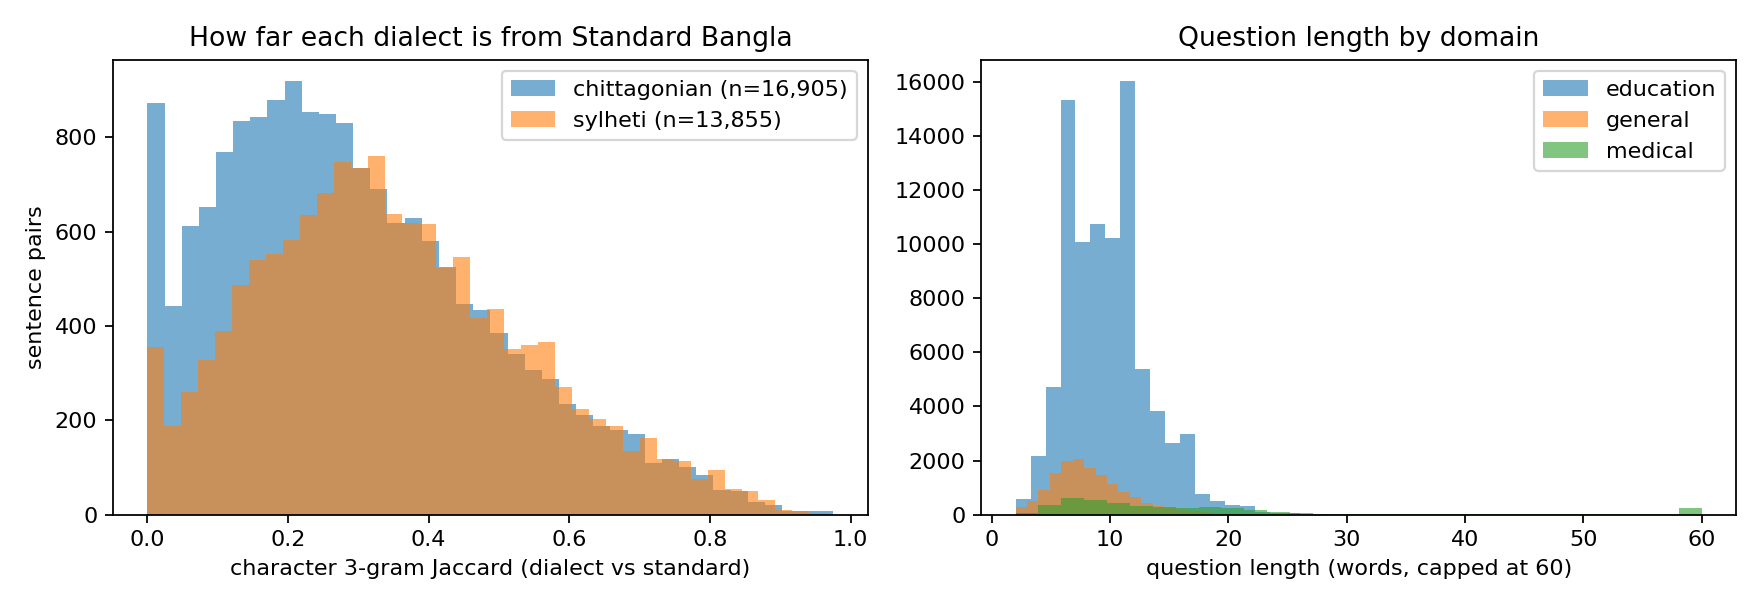
\includegraphics[width=0.66\textwidth]{fig_dialect_divergence.png}\hfill
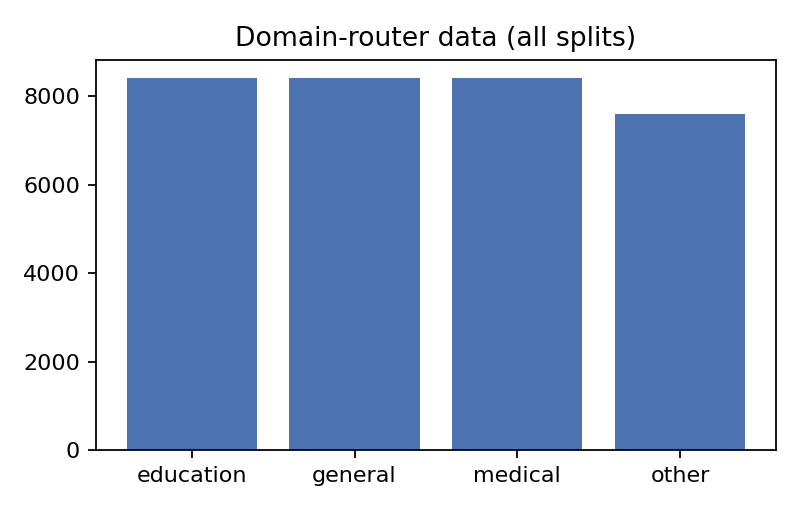
\includegraphics[width=0.30\textwidth]{fig_domain_distribution.png}
\caption{Left: character 3-gram Jaccard between each dialect sentence and its Standard translation (a peak near 0 means almost every trigram changed), and question length per domain. Right: the balanced domain-router data.}
\label{fig:divergence}
\end{figure}

\begin{figure}[!t]
\centering
\begin{tikzpicture}
\begin{axis}[width=\linewidth, height=40mm, ybar, bar width=9pt, ymin=0, ymax=60,
  symbolic x coords={Standard words kept,trigram containment,trigram Jaccard x100}, xtick=data,
  ylabel={\%}, enlarge x limits=0.25, legend style={at={(0.5,1.03)}, anchor=south}, legend columns=2,
  nodes near coords, nodes near coords style={font=\tiny, /pgf/number format/fixed, /pgf/number format/precision=1}]
\addplot[fill=amber, draw=none] coordinates {(Standard words kept,29.6) (trigram containment,43.0) (trigram Jaccard x100,29.6)};
\addplot[fill=navy, draw=none] coordinates {(Standard words kept,36.5) (trigram containment,49.4) (trigram Jaccard x100,34.8)};
\legend{Chittagonian, Sylheti}
\end{axis}
\end{tikzpicture}
\caption{How much of the Standard sentence survives in the dialect sentence (Bangla-script pairs, all splits).}
\label{fig:overlap}
\end{figure}

\subsection{Cleaning}
All text is Unicode-NFC normalized; invisible characters (zero-width space, soft hyphen, byte-order mark) are removed while the joiners Bangla needs are kept. Fig.~\ref{fig:cleaning} lists the removals. Word-level dictionary entries are removed from the \emph{training} pairs because the normalization expert rewrites whole questions, and 10k one-word examples would teach context-free word swaps and very short outputs; they were reused later, differently, as a glossary of 2,356 Chittagonian and 974 Sylheti entries (TRAIN split only), which was tested in system v2 (Section~\ref{sec:v2}). Pairs whose dialect text equals the Standard text carry no dialect signal and would give the dialect router the same sentence with two labels.

\begin{figure}[!t]
\centering
\resizebox{\linewidth}{!}{\begin{tikzpicture}
\begin{axis}[width=\linewidth, height=46mm, xbar, bar width=5pt, xmin=0, xmax=21500, xmode=normal,
  symbolic y coords={Mixed-script pair,Doctor answer too short,Doctor answer not Bangla script,Duplicate doctor question,Dialect text = Standard,Word-level lexicon entry,Duplicate dialect pair},
  ytick=data, xlabel={rows removed}, nodes near coords, nodes near coords style={font=\tiny},
  enlarge y limits=0.08, xmajorgrids, ymajorgrids=false, scaled x ticks=false]
\addplot[fill=greyd, draw=none] coordinates {(3,Mixed-script pair) (15,Doctor answer too short) (175,Doctor answer not Bangla script) (528,Duplicate doctor question) (546,Dialect text = Standard) (9989,Word-level lexicon entry) (17631,Duplicate dialect pair)};
\end{axis}
\end{tikzpicture}}
\caption{Cleaning log. Duplicates dominate: ChatgaiyyaBench re-distributes Vashantor and ChatgaiyyaAlap sentences. Doctor QA shrinks from 5,135 to 4,417 pairs.}
\label{fig:cleaning}
\end{figure}

\subsection{Transformation}
Every task becomes a chat instruction (system message, user message, target), written in Bangla so that the model answers in Bangla. Normalization prompts name the variety (``variety: Chittagonian; sentence: \ldots''); QA prompts contain three retrieved passages followed by the question. To teach grounded behaviour, the QA training targets follow the mix in Fig.~\ref{fig:mix}: 25\% of examples are real unanswerable questions and 8\% are \emph{retrieval misses} (the gold passage removed), both with a fixed ``the answer was not found in the given information'' target. Knowledge-base passages are split into overlapping windows of 110 words (stride 90) for NCTB-QA and BanglaRQA passages and 128 words for textbook rows (about 93--95 words on average); medical documents are stored as question--answer pairs or entity descriptions (about 27 words).

\begin{figure}[!t]
\centering
\begin{tikzpicture}
\begin{axis}[width=\linewidth, height=26mm, xbar stacked, bar width=10pt, xmin=0, xmax=100, ytick=\empty,
  xlabel={share of QA training examples (\%)}, legend style={at={(0.5,1.08)}, anchor=south, legend columns=3},
  ymajorgrids=false, xmajorgrids, nodes near coords, nodes near coords style={font=\tiny, text=white}]
\addplot[fill=navy, draw=none] coordinates {(67,0)};
\addplot[fill=amber, draw=none] coordinates {(25,0)};
\addplot[fill=redd, draw=none] coordinates {(8,0)};
\legend{answer in the evidence, unanswerable question, retrieval miss}
\end{axis}
\end{tikzpicture}
\caption{Target mix of the QA experts' training data: a third of the targets teach the expert to say ``not found'' instead of guessing (RAFT-style training \cite{zhang2024raft}).}
\label{fig:mix}
\end{figure}

\subsection{Integration, Splits and Reduction}
The dialect sources are merged into one pair table with provenance and split by \emph{group}: all versions of the same Standard sentence stay in one split (80/8/12), so no Standard sentence is seen in training and testing. Official splits (Vashantor, NCTB-QA, BanglaRQA, ChatgaiyyaBench benchmarks) are preserved, and a question text may never appear in two splits. Training sets are capped to fit the GPU budget: 24,000 normalization pairs, 11,943 education, 7,994 general and all 3,513 medical examples. Unverified silver data are used for training only. Table~\ref{tab:splits} gives the resulting splits and Table~\ref{tab:kb} the knowledge bases.

\begin{table}[!t]
\centering
\caption{Leak-free split sizes.}
\label{tab:splits}
\scriptsize
\begin{tabular}{@{}llrrr@{}}
\toprule
Task & Subset & Train & DEV & TEST \\
\midrule
\multirow{3}{*}{Dialect pairs} & Chittagonian & 16,030 & 1,411 & 1,968 \\
 & Sylheti & 13,119 & 1,295 & 1,961 \\
 & Standard (romanized) & 1,874 & 250 & 375 \\
\multirow{3}{*}{Dialect ID} & Chittagonian & 12,000 & 1,403 & 1,957 \\
 & Standard & 12,000 & 2,000 & 2,000 \\
 & Sylheti & 12,000 & 1,275 & 1,947 \\
Domain router & 4 classes & 6,000 each & 1,200 & 1,200 \\
\multirow{3}{*}{QA} & Education & 70,303 & 8,119 & 8,489 \\
 & General & 11,912 & 1,441 & 1,446 \\
 & Medical & 3,513 & 433 & 471 \\
MCQ (eval only) & 3 benchmarks & -- & 2,457 & 5,618 \\
Controller & 3 decisions & -- & 1,127 & 1,857 \\
\bottomrule
\end{tabular}
\end{table}

\begin{table}[!t]
\centering
\caption{Knowledge bases (searched, never trained on).}
\label{tab:kb}
\scriptsize
\resizebox{\linewidth}{!}{%
\begin{tabular}{@{}lrrr@{}}
\toprule
KB & Chunks & Documents & Avg.\ words \\
\midrule
Education (NCTB-QA passages + textbooks) & 163,591 & 96,907 & 93.2 \\
General (BanglaRQA passages) & 7,948 & 2,996 & 94.9 \\
Medical (doctor answers, MedER, drugs, intents) & 28,134 & 28,134 & 26.9 \\
Medical evaluation pool (retrieval benchmark only) & 904 & 904 & 48.7 \\
\bottomrule
\end{tabular}}
\end{table}

% =============================================================================
\section{Base-Model Selection}
\label{sec:models}

Seven open models were compared (Table~\ref{tab:candidates}): six instruction-tuned models and one Bangla base model. They include two \emph{Bangla-adapted vs.\ original} pairs (TigerLLM-1B \cite{raihan2025tigerllm} vs.\ Gemma-3-1B \cite{gemma3}; TituLM-3B \cite{titulm2025} vs.\ Llama-3.2-3B \cite{meta2024llama32}) to test whether Bangla continued pre-training still helps after task fine-tuning. The released TigerLLM-1B checkpoint has the architecture and tokenizer of Gemma-3-1B (identical fertility in Fig.~\ref{fig:fertility}), so Gemma-3-1B is its original model. Tokenizer fertility was measured first (Fig.~\ref{fig:fertility}): models that need 6--7 tokens per Bangla word make every example 4--5 times longer, which raises training time and forced a 4,096-token limit so that no long medical example is silently dropped.

\begin{table}[!t]
\centering
\caption{Candidate base models.}
\label{tab:candidates}
\scriptsize
\begin{tabular}{@{}lrc@{}}
\toprule
Model & Params (B) & Bangla-adapted \\
\midrule
TigerLLM-1B-it \cite{raihan2025tigerllm} & 1.0 & yes \\
Gemma-3-1B-it \cite{gemma3} & 1.0 & no \\
TituLM-Llama-3.2-3B \cite{titulm2025} & 3.2 & yes (base model) \\
Llama-3.2-3B-Instruct \cite{meta2024llama32} & 3.2 & no \\
Tiny-Aya-Fire \cite{tinyaya} & 3.35 & no \\
Qwen3-4B-Instruct-2507 \cite{qwen3} & 4.0 & no \\
Gemma-4-E4B-it \cite{gemma4} & 4.0 & no \\
\bottomrule
\end{tabular}
\end{table}

\begin{figure}[!t]
\centering
\begin{tikzpicture}
\begin{axis}[width=\linewidth, height=48mm, xbar, bar width=2.6pt, xmin=0, xmax=8,
  symbolic y coords={Gemma-4-E4B,Qwen3-4B,Tiny-Aya-Fire,Llama-3.2-3B,TituLM-3B,Gemma-3-1B,TigerLLM-1B},
  ytick=data, xlabel={tokens per word (lower = cheaper, longer context)}, enlarge y limits=0.1,
  legend style={at={(0.5,1.02)}, anchor=south}, legend columns=3, xmajorgrids, ymajorgrids=false, reverse legend]
\addplot[fill=greyd, draw=none] coordinates {(1.99,Gemma-4-E4B) (6.10,Qwen3-4B) (4.55,Tiny-Aya-Fire) (7.09,Llama-3.2-3B) (2.02,TituLM-3B) (1.99,Gemma-3-1B) (1.99,TigerLLM-1B)};
\addplot[fill=amber, draw=none] coordinates {(2.08,Gemma-4-E4B) (6.03,Qwen3-4B) (4.37,Tiny-Aya-Fire) (7.02,Llama-3.2-3B) (2.08,TituLM-3B) (2.08,Gemma-3-1B) (2.08,TigerLLM-1B)};
\addplot[fill=navy, draw=none] coordinates {(1.47,Gemma-4-E4B) (5.99,Qwen3-4B) (4.37,Tiny-Aya-Fire) (6.97,Llama-3.2-3B) (1.58,TituLM-3B) (1.47,Gemma-3-1B) (1.47,TigerLLM-1B)};
\legend{Sylheti, Chittagonian, Standard}
\end{axis}
\end{tikzpicture}
\caption{Tokenizer fertility on Standard, Chittagonian and Sylheti text. Dialect text costs 30--40\% more tokens than Standard text for the Gemma tokenizers.}
\label{fig:fertility}
\end{figure}

\textbf{Identical budget.} Every candidate receives the same QLoRA budget: 400 optimizer steps on the same 6,800 mixed-task examples, the same LoRA configuration, learning-rate schedule and seed. All candidates are evaluated zero-shot and after fine-tuning on a shared benchmark, and the choice uses a DEV composite
\begin{equation}
S=\tfrac{1}{5}\Big(\tfrac{\mathrm{chrF}_{\mathrm{ctg}}}{100}+\tfrac{\mathrm{chrF}_{\mathrm{syl}}}{100}+F1_{\mathrm{edu}}+F1_{\mathrm{gen}}+\tfrac{\mathrm{chrF}_{\mathrm{med}}}{100}\Big),
\end{equation}
where the first two terms are normalization quality and the rest are QA quality. The two finalists are re-trained with three seeds and compared with paired randomization tests; the winner (Gemma-4-E4B-it) hosts every expert.

% =============================================================================
\section{System Components}
\label{sec:components}

\subsection{Safety Layer}
Regular expressions written for Standard Bangla, Chittagonian, Sylheti and romanized Bangla detect emergencies (e.g.\ chest pain with breathlessness, unconsciousness, poisoning, stroke signs, suicidal statements) and dose or prescription requests. They run twice, on the raw and on the normalized question (Fig.~\ref{fig:safety}). Emergencies bypass the language model and return a fixed message asking the user to call the national emergency number 999 or go to the nearest hospital. No language model decides safety.

\begin{figure}[!t]
\centering
\resizebox{\linewidth}{!}{\begin{tikzpicture}[font=\tiny, node distance=3mm and 4mm]
\node[grey, text width=13mm] (q) {question};
\node[safe, right=of q, text width=15mm] (r1) {rules on raw text};
\node[lora, right=of r1, text width=13mm] (n) {normalize (if needed)};
\node[safe, right=of n, text width=15mm] (r2) {rules on normalized text};
\node[box, fill=redlt, draw=redd, below=4mm of r1, text width=15mm] (em) {emergency: fixed reply, no LLM};
\node[box, right=of r2, text width=14mm] (on) {continue pipeline};
\node[safe, below=4mm of on, text width=14mm] (out) {medical answer: dose refusal + referral note};
\draw[arr] (q) -- (r1); \draw[arr] (r1) -- (n); \draw[arr] (n) -- (r2); \draw[arr] (r2) -- (on); \draw[arr] (on) -- (out);
\draw[arr] (r1) -- (em); \draw[arr] (r2.south) |- (em.east);
\end{tikzpicture}}
\caption{Deterministic safety: emergency rules before and after normalization, and the output guard on every medical answer.}
\label{fig:safety}
\end{figure}

\subsection{Dialect Router and Normalization Trigger}
The dialect router classifies a question as Standard, Chittagonian or Sylheti from the union of character $n$-grams (1--5, word-bounded, robust to spelling variation) and word $n$-grams (1--2), weighted by TF-IDF, with a class-balanced linear SVM whose scores are calibrated with 3-fold sigmoid calibration; the regularisation constant $C$ is tuned on DEV macro-F1. Logistic regression, Complement Naive Bayes and single-feature variants are the alternatives, and a fine-tuned BanglaBERT \cite{bhattacharjee2022banglabert} tests whether a transformer router is worth its cost. The normalization trigger is
\begin{equation}
\mathrm{normalize}(q)=\big[v\neq\mathrm{Std}\wedge p_v\ge 0.45\big]\vee\big[q\ \text{is romanized}\big],
\end{equation}
so a Standard question is never rewritten unless the router is at least moderately sure it is dialectal.

\subsection{Normalization Expert}
The normalization expert is a LoRA adapter trained on 24,000 examples drawn from the training pairs in both directions: dialect or romanized $\rightarrow$ Standard (Chittagonian, Sylheti, and romanized input including romanized Standard Bangla) and Standard $\rightarrow$ dialect. The variety is named in the prompt; 15\% of dialect prompts carry a generic ``regional Bangla'' label instead, so the expert also works when the router is unsure. It was trained for one epoch (1,500 steps) and, as a DEV-selected improvement, re-trained for two epochs; the two-epoch expert was adopted because it was better on DEV (78.67 vs.\ 77.24 chrF++). The reverse direction is used only to build the paired test set (Section~\ref{sec:paired}). When the expert's mean token log-probability for a rewrite is below $-0.9$, the system shows its interpretation and asks the user to confirm it.

\textbf{Baselines.} Zero-shot prompting of the base model, and 5-shot prompting whose examples are the five most similar training pairs (character 2--4-gram TF-IDF, same variety and script), a stronger baseline than fixed examples; the BanglaCHQ-Prantik metric set \cite{prantik2025} is reported next to chrF++. A LoRA expert on a 16-bit base with identical data, steps and seed answers the LoRA-vs-QLoRA question.

\subsection{Domain Router}
The domain router uses the same features and classifier over four classes (education, general, medical, other), trained on 6,000 balanced questions per class. It runs on the \emph{normalized} question, so dialect words do not confuse it.

\subsection{Answer / Clarify / Abstain Controller}
The controller decides whether to answer, ask for clarification or abstain from 20 features (Fig.~\ref{fig:controller}). Logistic regression and gradient-boosted trees \cite{friedman2001gbm} are compared with 5-fold cross-validation on DEV (macro-F1). Its data combine clear in-scope questions (ANSWER), out-of-scope sentences (ABSTAIN) and constructed under-specified questions such as a symptom without context (CLARIFY). Abstention because the \emph{evidence} lacks the answer is not the controller's job: the experts learn it from real unanswerable questions.

\begin{figure}[!t]
\centering
\begin{tikzpicture}[font=\tiny, node distance=2mm]
\node[box, text width=24mm] (f1) {3 dialect + 4 domain probabilities; top domain probability and margin};
\node[cpu, text width=24mm, below=of f1] (f2) {BM25 signals: log top score, gap to 2nd passage, best score over all KBs};
\node[grey, text width=24mm, below=of f2] (f3) {text: words, content words, vagueness, question word / mark, romanized, medical entities, length};
\node[box, fill=navy, text=white, right=7mm of f2, text width=15mm, minimum height=12mm] (gb) {gradient-boosted trees};
\node[box, right=7mm of gb, yshift=6mm, text width=16mm] (a) {ANSWER};
\node[grey, right=7mm of gb, text width=16mm] (c) {CLARIFY};
\node[safe, right=7mm of gb, yshift=-6mm, text width=16mm] (b) {ABSTAIN};
\draw[arr] (f1.east) -- (gb); \draw[arr] (f2) -- (gb); \draw[arr] (f3.east) -- (gb);
\draw[arr] (gb) -- (a); \draw[arr] (gb) -- (c); \draw[arr] (gb) -- (b);
\end{tikzpicture}
\caption{The controller's 20 features and its three decisions.}
\label{fig:controller}
\end{figure}

\subsection{Retrieval per Domain}
Each domain has its own knowledge base. Four retriever families are compared on DEV (Standard questions, document-level nDCG@10): BM25, character TF-IDF, dense retrieval with BGE-M3 or multilingual-E5-base, and hybrids fused by RRF (Eq.~\ref{eq:rrf}). The retriever is chosen \emph{per domain}; a dense method is taken only if it beats the best sparse method by at least 0.01 nDCG@10, because dense search costs GPU time. The result is BM25 for education and general knowledge and dense BGE-M3 for medicine. The expert receives the top $k=3$ passages (at most 600 characters each, 1,800 in total).

\textbf{Dialect-invariant encoder.} As a novel variant, BGE-M3 is fine-tuned so that a dialect sentence $x_i$ and its Standard translation $y_i$ embed close together, with the symmetric InfoNCE loss \cite{oord2018cpc} over a batch of $B=32$ pairs:
\begin{equation}
\mathcal{L}=-\frac{1}{2B}\sum_{i=1}^{B}\Big[\log\frac{e^{s_{ii}/\tau}}{\sum_j e^{s_{ij}/\tau}}+\log\frac{e^{s_{ii}/\tau}}{\sum_j e^{s_{ji}/\tau}}\Big],
\end{equation}
where $s_{ij}=\cos(\mathbf{e}_{x_i},\mathbf{e}_{y_j})$,
$\tau=0.05$, 600 steps and learning rate $2\times10^{-5}$. Every third batch replays (question, gold passage) pairs so that retrieval ability is not forgotten; the encoder is evaluated exactly like the others.

\subsection{Routed Experts and the Pooled Control}
Three answer experts (education, general, medical) are trained on their domain's QA data with three retrieved passages in the prompt (Table~\ref{tab:train}). As a control, one \emph{pooled} adapter is trained on the union of all expert data with the same total number of optimizer steps as all experts together (3,184 steps, 317 vs.\ 316 minutes), so ``routed experts vs.\ one adapter'' is compared at equal compute. Table~\ref{tab:hyper} lists the shared hyper-parameters.

\begin{table}[!t]
\centering
\caption{Adapters trained on Gemma-4-E4B-it (QLoRA unless stated).}
\label{tab:train}
\scriptsize
\begin{tabular}{@{}lrrrr@{}}
\toprule
Adapter & Examples & Steps & Minutes & Peak GB \\
\midrule
Normalization & 24,000 & 1,500 & 72.9 & 19.9 \\
Education & 11,943 & 746 & 112.6 & 30.3 \\
General & 7,994 & 499 & 76.0 & 29.1 \\
Medical (2 epochs) & 3,513 & 439 & 54.9 & 34.7 \\
Pooled (all data) & 47,450 & 3,184 & 316.6 & 34.7 \\
Normalization, LoRA 16-bit & 24,000 & 1,500 & 60.0 & 18.1 \\
\bottomrule
\end{tabular}
\end{table}

\begin{table}[!t]
\centering
\caption{Shared training and decoding settings.}
\label{tab:hyper}
\scriptsize
\begin{tabularx}{\linewidth}{@{}L{2.9cm} Y@{}}
\toprule
Setting & Value \\
\midrule
Base model & Gemma-4-E4B-it, 4-bit NF4, double quantization, BF16 compute \\
LoRA & $r=16$, $\alpha=32$, dropout 0.05, all attention and MLP projections \\
Optimizer & AdamW \cite{loshchilov2019adamw}, learning rate $2\times10^{-4}$, 3\% warm-up, cosine decay \\
Batch & 4 examples $\times$ 4 accumulation steps = 16 \\
Sequence limit & 4,096 tokens (0 examples dropped) \\
Seed & 17 (finalists of S2: 17, 42, 101) \\
Decoding & greedy; 96 new tokens for normalization (up to 384 for long questions), 64 for education/general, 200 for medical \\
Evidence & $k=3$ passages, best first \\
\bottomrule
\end{tabularx}
\end{table}

% =============================================================================
\section{Evaluation Protocol}
\label{sec:eval}

\subsection{Metrics}
\textbf{Normalization} uses chrF++ as the primary metric \cite{popovic2017chrfpp}, because character $n$-grams tolerate the spelling variation typical of dialects:
\begin{equation}
\mathrm{chrF}_\beta=(1+\beta^2)\frac{\mathrm{chrP}\cdot\mathrm{chrR}}{\beta^2\,\mathrm{chrP}+\mathrm{chrR}},\quad\beta=2,
\end{equation}
where chrP and chrR are the character $n$-gram ($n\le6$) precision and recall; chrF++ adds word unigrams and bigrams. BLEU \cite{papineni2002bleu} (computed with sacreBLEU \cite{post2018sacrebleu}), character error rate and, for comparisons with published work, ROUGE \cite{lin2004rouge} and METEOR \cite{banerjee2005meteor} are reported as well.

\textbf{Extractive QA} (education, general) uses exact match and token F1:
\begin{equation}
F1=\frac{2PR}{P+R},\quad P=\frac{|\hat a\cap a|}{|\hat a|},\ R=\frac{|\hat a\cap a|}{|a|},
\end{equation}
over the bags of tokens of the predicted answer $\hat a$ and the gold answer $a$ (maximum over gold answers). \textbf{Medical} answers use chrF++ and ROUGE-L against the doctor's answer, plus the referral rate and the share of answer words found in the evidence. \textbf{Retrieval} uses hit@$k$, MRR@10 and nDCG@10 at document level, and \emph{answer-containment} hit@$k$ (the gold answer string occurs in the top-$k$ passages). \textbf{Routers} use accuracy, macro-F1 and ECE.

The end-to-end \textbf{QA score} of a question is its token F1 (education, general) or chrF++/100 (medical), and 0 when an answerable question is not answered; behaviour is scored separately (answered share, correct abstention on unanswerable and out-of-scope questions, clarification on vague ones). The \textbf{dialect gap} is $g_v=\mathrm{QA}_{\mathrm{Std}}-\mathrm{QA}_v$, and the share of the gap a system closes is
\begin{equation}
\mathrm{closed}_v=\frac{g_v^{\,\mathrm{NO\_NORM}}-g_v^{\,\mathrm{system}}}{g_v^{\,\mathrm{NO\_NORM}}}.
\end{equation}

\subsection{Statistics}
All tables report 95\% percentile-bootstrap confidence intervals over test items \cite{efron1993bootstrap,koehn2004bootstrap}. Two systems evaluated on the same items are compared with a paired approximate-randomization test \cite{riezler2005randomization}: the per-item scores of the two systems are randomly swapped 2,000--5,000 times, and $p$ is the share of swaps whose mean difference is at least as large as the observed one. The full system is compared with seven ablations in three varieties plus the oracle, giving 22 $p$-values, which are corrected with the Holm procedure \cite{holm1979}: with $p_{(1)}\le\dots\le p_{(m)}$, the $i$-th hypothesis is rejected while $p_{(i)}\le\alpha/(m-i+1)$.

\subsection{Paired End-to-End Test Set}
\label{sec:paired}
Dialect QA test data with reference answers do not exist. We therefore take 780 test questions (200 each from education, general and medical, plus 60 unanswerable, 60 out-of-scope and 60 under-specified), rewrite each into Chittagonian and Sylheti with the reverse direction of the normalization expert, and keep a dialect version only if it differs from the original and a round trip back to Standard reaches chrF++ $\ge 40$ (Fig.~\ref{fig:paired}). 92.3\% of the Chittagonian and 92.9\% of the Sylheti versions were kept, giving 2,225 questions: the \emph{same} questions in three varieties, so any score difference is caused by the variety alone.

\begin{figure}[!t]
\centering
\begin{tikzpicture}[font=\tiny, node distance=3mm and 4mm]
\node[grey, text width=15mm] (s) {780 Standard TEST questions};
\node[lora, right=of s, text width=14mm] (d) {Std $\rightarrow$ dialect (reverse direction)};
\node[lora, right=of d, text width=14mm] (b) {back to Standard};
\node[box, right=of b, text width=14mm] (f) {keep if changed and round-trip chrF++ $\ge$ 40};
\node[cpu, below=4mm of d, text width=40mm] (o) {2,225 paired questions: 780 Standard, 720 Chittagonian, 725 Sylheti $\Rightarrow$ 9 system conditions};
\draw[arr] (s) -- (d); \draw[arr] (d) -- (b); \draw[arr] (b) -- (f); \draw[arr] (f.south) |- (o.east);
\end{tikzpicture}
\caption{Building the paired test set. Because the dialect versions are model-written and ``lighter'' than real dialect text, a second evaluation uses 481 questions written by native speakers (Section~\ref{sec:human}).}
\label{fig:paired}
\end{figure}

\subsection{Human-Written Dialect Questions}
\label{sec:human}
The question sentences in the held-out test split of the native-written parallel corpora (Kothon, Vashantor, ChatgaiyyaAlap, ONUBAD) give 481 real dialect questions (234 Chittagonian, 247 Sylheti), each with its human Standard translation but without a reference answer. The system is therefore evaluated by \emph{consistency}: does it treat the dialect question like its Standard version (same decision, same domain, similar answer, overlapping evidence)?

\subsection{Ablation Conditions}
Table~\ref{tab:conditions} lists the nine conditions run on the paired test set. Each removes or replaces one component, so the difference to \cond{FULL} measures that component's contribution.

\begin{table}[!t]
\centering
\caption{End-to-end evaluation conditions.}
\label{tab:conditions}
\scriptsize
\begin{tabularx}{\linewidth}{@{}L{2.75cm} Y L{1.3cm}@{}}
\toprule
Condition & What is changed & Answers \\
\midrule
\condt{FULL} & nothing (proposed system) & per variety \\
\condt{NO\_NORMALIZATION} & dialect text goes straight to routing, retrieval, expert & RQ2 \\
\condt{ALWAYS\_NORMALIZE} & dialect router bypassed; everything normalized & router value \\
\condt{NO\_DOMAIN\_ROUTING} & one merged KB and the pooled adapter & RQ3 \\
\condt{POOLED\_ADAPTER} & routed experts $\rightarrow$ one pooled adapter & RQ3 \\
\condt{BASE\_MODEL} & no fine-tuning (same prompts) & RQ3 \\
\condt{NO\_RAG} & closed-book answering & RQ3 \\
\condt{NO\_CONTROLLER} & always answer & RQ3 \\
\condt{ORACLE\_STANDARD} & gold Standard question and domain & upper bound \\
\bottomrule
\end{tabularx}
\end{table}

\subsection{Comparability with Published Work}
To compare with published dialect-translation models, the normalization expert is also scored on the \emph{official} Vashantor test sentences \cite{faria2023vashantor} with the papers' own metrics (BLEU, BLEU-1, chrF, METEOR, WER, CER) and 95\% bootstrap intervals; an audit confirms that these sentences are the official test split and never occur in training. The QA experts are compared with the gold-passage results of BanglaRQA and NCTB-QA on the subset of questions whose gold passage was retrieved.

\subsection{Answer-Time Improvements (System v2)}
\label{sec:v2}
After the main results were frozen, a set of improvements that change only \emph{how} the trained models are used was defined (Table~\ref{tab:v2}, Fig.~\ref{fig:v2}). Each was switched on only if it improved the DEV split by a fixed margin (0.005 for retrieval and QA scores). The paired TEST set was then answered once more: a run with every change switched off, on 300 sampled test questions, checks that the v2 code reproduces the reported answers (validity check), and the adopted changes are added one at a time so that each step has its own paired test. The main results stay as reported; v2 is an extension.

The last column of Table~\ref{tab:v2} records the DEV decisions. Three changes were adopted: re-ranking of 50 candidates for education and general questions, with near-duplicate removal for education only (I4); searching both the education and the general knowledge base when the domain router's confidence is below $\tau=0.9$, which happened for about 46\% of DEV questions (I5); and the routing-independent medical note (I3). The other five were tested and not adopted, because they did not reach the DEV margin. The glossary helped Chittagonian but hurt Sylheti. Dual-query retrieval changed answer containment by less than 0.005. A forced second decoding did not raise the DEV QA score for any threshold. Repetition trimming lowered it slightly. The trigger chosen on DEV was the S5 rule itself.

\begin{table}[!t]
\centering
\caption{Answer-time improvements (no retraining), each chosen on DEV.}
\label{tab:v2}
\scriptsize
\begin{tabularx}{\linewidth}{@{}l Y L{2.0cm} L{3.1cm}@{}}
\toprule
& Change & DEV criterion & DEV decision \\
\midrule
I1 & also normalize ``Standard'' predictions with confidence $<t$ & Youden's $J$ \cite{youden1950index} on dialect-ID DEV & not adopted: the S5 rule had the highest $J$ (0.958) \\
I3 & medical note and dose refusal whenever a medical signal fires, independent of routing & F2 on domain DEV & \textbf{adopted}: domain-router medical probability $\ge 0.2$ \\
I4 & 50 candidates, near-duplicate removal \cite{lee2022dedup}, cross-encoder re-ranking \cite{nogueira2019passage,bgereranker2024} & answer-containment hit@3 & \textbf{adopted}: education re-rank + de-duplication (0.730 $\rightarrow$ 0.812); general re-rank (0.727 $\rightarrow$ 0.749) \\
I5 & search education and general KBs when the domain router's confidence $<\tau$ \cite{lee2025routerretriever} & answer-containment hit@3 & \textbf{adopted}: $\tau=0.9$ (0.697 $\rightarrow$ 0.767) \\
I6 & when the expert says ``not found'', decode again with that sentence blocked; keep it if mean log-prob.\ $\ge\theta$ & DEV QA, abstention $-5$ pts max & not adopted: DEV QA unchanged (0.540) at every $\theta$ \\
I7 & cut an answer where it starts repeating itself \cite{xu2022ditto} & DEV QA not lower & not adopted: 0.540 $\rightarrow$ 0.539 \\
I8 & dialect glossary (word entries, TRAIN split) shown to the normalization expert as example turns & chrF++ $\ge$ +0.5, no variety lower & not adopted: Chittagonian $+0.55$, Sylheti $-0.73$ \\
I9 & retrieve with original \emph{and} normalized question, fused by RRF \cite{rackauckas2024ragfusion} & hit@3 on dialectized DEV & not adopted: mean gain $<0.005$ \\
\bottomrule
\end{tabularx}
\end{table}

\begin{figure}[!t]
\centering
\begin{tikzpicture}[font=\tiny, node distance=2.5mm and 3.5mm]
\node[grey, text width=12mm] (q) {original question};
\node[lora, below=of q, text width=16mm] (n) {normalized (+ I8 glossary)};
\node[cpu, right=of q, text width=12mm] (c1) {50 cand.\ own KB};
\node[cpu, right=of n, text width=12mm] (c2) {50 cand.\ own KB};
\node[cpu, below=of c2, text width=12mm, dashed] (c3) {50 cand.\ other KB (I5, if unsure)};
\node[box, right=6mm of c2, text width=12mm, yshift=4mm] (f) {RRF fusion (I9)};
\node[box, right=of f, text width=13mm] (d) {near-duplicate removal (I4)};
\node[box, fill=navy, text=white, right=of d, text width=12mm] (r) {cross-encoder re-rank (I4)};
\node[box, below=of r, text width=12mm] (t) {top-3 $\rightarrow$ expert};
\draw[arr] (q) -- (c1); \draw[arr] (n) -- (c2); \draw[darr] (n.south) |- (c3.west);
\draw[arr] (c1.east) -- (f); \draw[arr] (c2.east) -- (f); \draw[darr] (c3.east) -- (f);
\draw[arr] (f) -- (d); \draw[arr] (d) -- (r); \draw[arr] (r) -- (t);
\end{tikzpicture}
\caption{Retrieval in system v2 as designed. After the DEV decisions (Table~\ref{tab:v2}), the adopted path is: normalized question $\rightarrow$ 50 candidates from the domain's KB, plus 50 from the other KB when the domain router's confidence is below 0.9 (I5) $\rightarrow$ near-duplicate removal (education) $\rightarrow$ cross-encoder re-ranking $\rightarrow$ top 3. The glossary (I8) and RRF fusion (I9) were tested but not adopted.}
\label{fig:v2}
\end{figure}

% =============================================================================
\section{Implementation Environment}
\label{sec:impl}
The implementation is a Python 3.12 library of 20 modules (data, metrics, retrieval, routers, prompts, training and inference, pipeline, analysis, reporting) embedded in the stage notebooks, so each notebook runs on a fresh machine. The GPU stack is PyTorch 2.8 (CUDA 12.8), Hugging Face Transformers 4.57 (and 5.x in a second environment for Gemma-4), PEFT 0.21, bitsandbytes 0.50 and Accelerate 1.15; the CPU stack adds scikit-learn 1.6 and sacreBLEU 2.5. GPU jobs run detached with atomic checkpoints (adapter, optimizer, scheduler, data order and random states), so a stopped machine resumes where it stopped. Fig.~\ref{fig:gpu} shows the GPU time per stage.

\begin{figure}[!t]
\centering
\resizebox{\linewidth}{!}{\begin{tikzpicture}
\begin{axis}[width=\linewidth, height=36mm, xbar, bar width=5pt, xmin=0, xmax=21,
  symbolic y coords={S10 system v2,S6 human-written + demo,S5 system + 9 conditions,S4 dense retrieval,S3 experts,S2 model comparison},
  ytick={S10 system v2,S6 human-written + demo,S5 system + 9 conditions,S4 dense retrieval,S3 experts,S2 model comparison}, xlabel={A40 GPU-hours}, nodes near coords, nodes near coords style={font=\tiny}, bar shift=0pt,
  enlarge y limits=0.12, xmajorgrids, ymajorgrids=false]
\addplot[fill=navy, draw=none] coordinates {(18,S2 model comparison) (14.5,S3 experts) (1,S4 dense retrieval) (5.5,S5 system + 9 conditions) (1,S6 human-written + demo)};
\addplot[fill=greyd, draw=none] coordinates {(2,S10 system v2)};
\end{axis}
\end{tikzpicture}}
\caption{GPU time per stage: about 40 A40 GPU-hours ($\approx$US\$20 at US\$0.49/h) up to S6; system v2 added about 2 more hours.}
\label{fig:gpu}
\end{figure}

% =============================================================================
\section{Summary}
The methodology turns a Standard-only QA problem into a dialect-aware one with small, inspectable parts: a CPU dialect router decides \emph{whether} to rewrite, one LoRA expert rewrites, a CPU domain router and controller decide \emph{where} and \emph{whether} to answer, each domain retrieves its own evidence, and one LoRA expert per domain answers from it on a single shared 4-bit model, with deterministic rules for emergencies and medicines. Every decision is made on validation data, every result is reported per language variety, and the evaluation isolates the effect of each component: the same questions in three varieties, nine conditions with Holm-corrected paired tests, native-speaker questions, comparisons with published work on the same test sentences, and a DEV-selected set of answer-time improvements. Chapter~5 reports the results.

